% ============================================================
\chapter{$\tau$ の意味と決め方}\label{ch:tau}

$\tau$ は、BL でいちばん誤解されやすい係数である。Walters は、$\tau$ の意味と効き方が多くの利用者を混乱させている、と書いている。文献に出てくる値も 0.01 から 1 まで幅がある。この章では、$\tau$ が何を表し、いつ効いていつ消えるのかを整理し、決め方の選択肢を比べる。

\section{$\tau$ の 2 つの役割}

$\tau$ は 2 か所に出てくる。

\begin{enumerate}
\item \textbf{混ぜ方}：事後の期待リターン $\muBL=\Pi+\tau\Sigma P\T(P\tau\Sigma P\T+\Omega)^{-1}(Q-P\Pi)$ では、$\tau\Sigma$ と $\Omega$ の比として効く。
\item \textbf{事後の不確かさ}：$M=\tau\Sigma-\cdots$ と、予測の共分散 $\Sigma+M$ では、$\tau$ そのものの大きさが効く。
\end{enumerate}

1 番目の役割では比だけが効くので、$\Omega$ をどう決めるかによって、$\tau$ が効いたり消えたりする。2 番目の役割は、最適化で $\Sigma+M$ を使うときだけ効く。

\section{文献に出てくる値}

\begin{table}[htbp]
\centering
\caption{文献での $\tau$ の値と決め方。}
\label{tab:tau-lit}
\small
\begin{tabular}{p{3.8cm}p{2.6cm}p{6.6cm}}
\toprule
文献 & 値 & 考え方 \\
\midrule
Black and Litterman（1992） & 0 に近い値 & 平均の不確かさはリターンの不確かさよりずっと小さい（Idzorek による紹介） \\
Lee（2000） & 0.01〜0.05 & そのうえで、目標のトラッキングエラーに合うように調整する（Idzorek による紹介） \\
He and Litterman（1999） & 0.05 & $\Omega=\tau\diag(P\Sigma P\T)$ と組み合わせる \\
Idzorek（2007） & 0.025 & 同上。確信度の方法では $\tau$ は結果に効かない \\
Satchell and Scowcroft（2000） & 1 がよく使われる & $\tau$ を確率変数とするモデルも提案 \\
Blamont and Firoozye（2003） & $\approx1/T$ & $\tau\Sigma$ を均衡リターンの推定の標準誤差とみる \\
Meucci（2010） & $\approx1/T$ & 実際には (0, 1) の範囲で用途に合わせて調整。数値例は 0.4 \\
PyPortfolioOpt & 0.05（既定） & 既定の $\Omega$ や Idzorek の方法では $\tau$ は消える \\
対象論文（Lee ほか 2025、第 2 版） & 検証期間で選ぶ & $\tau_{\mathrm{init}}=$ 平均($\Omega$) ÷ 平均($\Sigma$) を中心に 0.5〜1.5 倍の 5 点からシャープレシオで選ぶ \\
本プロジェクト & 0.025 & 元論文の第 1 版に合わせた \\
O'Toole（2017） & 調整する & $\tau$ は暗黙のアクティブリスクの大きさと直結しており、目標のアクティブリスクに合わせて決められる \\
Allaj（2013） & 推定する & 横断面と時系列の回帰から $\tau$ を推定する \\
\bottomrule
\end{tabular}
\end{table}

\tabref{tab:tau-lit} の値は 2 桁近く違う。しかし、多くの場合、$\Omega$ の決め方と組み合わせると、結果の違いは見た目ほど大きくない。次の節で理由を見る。

\section{$\Omega$ を $\tau$ に比例させると、$\tau$ は消える}\label{sec:tau-cancel}

He と Litterman は $\Omega=\tau\diag(P\Sigma P\T)$ と置いた。$\Omega$ が $\tau$ に比例していれば、$\Omega=\tau\Omega_0$ と書ける。更新形に入れると、
\begin{equation}
\muBL=\Pi+\tau\Sigma P\T\bigl(\tau P\Sigma P\T+\tau\Omega_0\bigr)^{-1}(Q-P\Pi)
=\Pi+\Sigma P\T\bigl(P\Sigma P\T+\Omega_0\bigr)^{-1}(Q-P\Pi)
\label{eq:tau-cancel}
\end{equation}
となり、$\tau$ は約分されて消える。Idzorek は、$\tau$ を 0.025 から 15 に変えても事後の期待リターンが変わらないことを、例で確かめている。PyPortfolioOpt の説明にも、既定の $\Omega$ や Idzorek の方法では「$\tau$ の値は効かない」と書かれている。

\begin{table}[htbp]
\centering
\caption{Idzorek の例で $\tau$ を変えたときの、先進国株式の事後の期待リターン $\mu$ と、その不確かさ $\sqrt{M}$（年率 \%）。左の 2 列は $\Omega=\tau\diag(P\Sigma P\T)$（$\tau$ に比例）、右の 3 列は $\Omega$ を $\tau=0.025$ のときの値に固定したもの。「$Q$ への移動」は、均衡 4.80\% からビュー 5.25\% までの何割動いたか。}
\label{tab:tau}
\tabin{tau}
\end{table}

\tabref{tab:tau} の左の 2 列のとおり、$\Omega$ を $\tau$ に比例させると、事後の期待リターンは $\tau$ によらず同じである。変わるのは事後の不確かさ $\sqrt{M}$ だけで、$\sqrt\tau$ に比例して大きくなる。

\section{$\Omega$ を固定すると、$\tau$ が採用率を決める}

$\Omega$ を $\tau$ と無関係に決めると、話が変わる。\tabref{tab:tau} の右の 3 列と\figref{fig:tau}は、$\Omega$ を固定して $\tau$ だけを動かした結果である。$\tau$ が小さいと均衡のまま、大きいとビューのほうへ動く。

\begin{figure}[htbp]
\centering
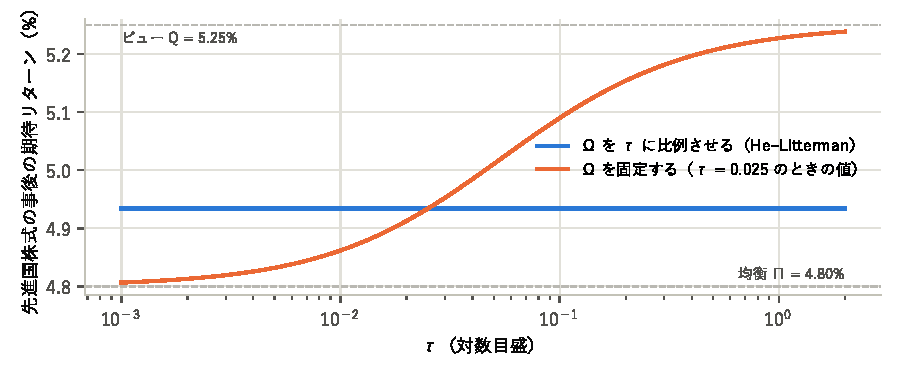
\includegraphics[width=0.92\linewidth]{fig_tau.pdf}
\caption{Idzorek の例で $\tau$ を動かしたときの、先進国株式の事後の期待リターン。$\Omega$ を $\tau$ に比例させると（青）一定、$\Omega$ を固定すると（橙）$\tau$ とともにビューへ近づく。}
\label{fig:tau}
\end{figure}

$\Omega$ を外から決める方法は多い。予想の誤差の分散、モデルの条件付き分散、LLM の回答のばらつきなどである（\chapref{ch:omega}）。そのどれでも、$\tau$ はビューの採用率を直接決める係数になる。本プロジェクトの $\tau=0.025$ も、そういう係数として働いている。

対象論文の第 2 版は、検証用の 3 か月で $\tau$ を選び直している。出発点の $\tau_{\mathrm{init}}$ は、$\Omega$ の平均と $\Sigma$ の平均の比である。1 資産で考えると、$\tau=\omega/\sigma^2$ なら採用率はちょうど 50\% になるので、$\tau_{\mathrm{init}}$ は「採用率がおよそ半分になる $\tau$」である。そこから 0.5〜1.5 倍の 5 点を試し、シャープレシオがいちばん高いものを使う。考え方は理解できるが、3 か月（隔週の見直しで約 6 回）の成績で選ぶと、偶然の当たり外れに合わせてしまうおそれが大きい。

\section{$\tau\approx1/T$ の意味}

過去 $T$ 期のリターンから平均を推定すると、その推定値の共分散は $\Sigma/T$ である。均衡リターンを「$T$ 期分のデータで推定した平均と同じくらい確か」とみなせば、$\tau\Sigma=\Sigma/T$、つまり $\tau=1/T$ になる。

\begin{center}
\small
\begin{tabular}{lll}
\toprule
$\tau$ & 年次のデータに直すと & 月次のデータに直すと \\
\midrule
0.05 & 20 年分 & 1 年 8 か月分 \\
0.025 & 40 年分 & 3 年 4 か月分 \\
0.01 & 100 年分 & 8 年 4 か月分 \\
1 & 1 年分 & 1 か月分 \\
\bottomrule
\end{tabular}
\end{center}

ここで、$\Sigma$ の期間（年次か月次か）によって読み方が変わることに注意する。$\tau=0.025$ は、年率の $\Sigma$ と組み合わせれば「40 年分の年次データと同じ確かさ」、月次の $\Sigma$ と組み合わせれば「40 か月分の月次データ」である。$\tau\Sigma$ の大きさ（期待リターンの不確かさの分散）は、どちらも同じで、年率に直すと標準偏差で $\sqrt{0.025}\times20\%\approx3.2\%$（市場の年率の標準偏差を 20\% とした場合）である。「均衡リターンの見込みが年率 ±3\% 程度は外れうる」という程度の確かさで、感覚的にも妥当な水準である。

$\tau=1$ は、均衡リターンが 1 期分のリターンと同じくらい不確かという意味で、年率なら「期待リターンは ±20\% 外れうる」と言っていることになる。均衡をほとんど信じない設定で、ビューが強く効く。

\section{$\tau$ と事後の共分散}

最適化で $\Sigma+M$ を使う場合、$\tau$ は比率の大きさにも効く。ビューがないとき $\Sigma+M=(1+\tau)\Sigma$ なので、比率は $\wmkt/(1+\tau)$ になる。$\tau=0.05$ なら 95.2\%、$\tau=1$ なら 50\% しか危険資産に投資しない。Meucci は、この「ビューのない事後が事前と一致しない」性質をパズルとして取り上げ、ビューを期待値ではなく実現値についてのものと読み替えた市場版の BL で解いた（\chapref{ch:hlmeucci}）。市場版では $\tau$ がそもそも出てこない。

\section{$\tau$ でトラッキングエラーを合わせる}\label{sec:tau-te}

Idzorek は、Lee（2000）が $\tau$ を 0.01〜0.05 に置いたうえで、目標のトラッキングエラー（ベンチマークからのずれの標準偏差）に合うように調整している、と紹介している。O'Toole（2017）も、$\tau$ は BL に暗黙に含まれるアクティブリスクの大きさと直接つながっており、目標のアクティブリスクから $\tau$ を決められる、と論じている。

$\Omega$ を固定して $\tau$ を動かせば、ビューの採用率が変わり、比率の傾きの大きさ（トラッキングエラー）が変わる。Idzorek の例で計算すると（\figref{fig:te} の左）、$\tau=0.025$ のときのトラッキングエラーは年率 \V{te.tau.base}\% で、2\% に合わせるには $\tau\approx\V{te.tau2}$ が必要になる。

この決め方の利点は、意味の分かりにくい $\tau$ を、運用で意味のある量（ずれの許容幅）に置き換えられることである。欠点は、「どれだけずれてよいか」と「ビューをどれだけ信じるか」を混ぜてしまうことである。ビューの当たり具合が悪いのに、許容幅が大きいからといって採用率を上げるのは筋が悪い。当たり具合は $\Omega$ で、ずれの許容幅は最適化の制約で、別々に決めるほうがよい（\chapref{ch:te}）。

\section{2 つの参照モデル}

Walters の整理では、BL の使い方には大きく 2 つの流儀がある。

\begin{description}[leftmargin=2em,style=nextline]
\item[標準的な参照モデル] $\mu$ を確率変数とし、$\mu\sim\mathcal N(\Pi,\tau\Sigma)$ を真面目に使う。事後の共分散 $\Sigma+M$ で最適化する。$\tau$ の大きさそのものが意味を持つので、慎重に決める必要がある。
\item[もう 1 つの参照モデル] 事後の期待リターンだけを使い、最適化には $\Sigma$ を使う。$\Omega$ を $\tau$ に比例させることが多く、その場合 $\tau$ は結果に効かない。
\end{description}

実務の多く（Idzorek、PyPortfolioOpt、本プロジェクト）は後者である。後者を使うなら、「$\tau$ は何がよいか」と悩む必要はほとんどない。悩むべきは $\Omega$（または、$\Omega$ を固定したときの $\tau\Sigma$ との比）である。

\begin{tipbox}[コツ：$\tau$ の決め方]
\begin{enumerate}
\item まず、$\Omega$ を何に比例させるかを決める。$\Omega$ を $\tau P\Sigma P\T$ に比例させるなら、$\tau$ はどの値でもよい（0.025 か 0.05 で十分）。
\item $\Omega$ を外から決める（誤差の分散、回答のばらつき、モデルの分散など）なら、$\tau$ は採用率を決める係数である。採用率が当たり具合に見合う大きさになるように、$\tau$（または $\Omega$ の倍率）を決める（\chapref{ch:accuracy}）。
\item 最適化で $\Sigma+M$ を使うなら、$\tau$ は比率の大きさにも効く。$\tau=1$ のような大きな値は避ける。
\item 少ない期間の成績で $\tau$ を選ばない。選んだ $\tau$ が、採用率としてどれくらいの値になっているかを確かめる。
\end{enumerate}
\end{tipbox}

\begin{keybox}[この章のまとめ]
\begin{itemize}
\item $\tau$ は、混ぜ方では $\Omega$ との比として、事後の共分散では大きさそのものとして効く。
\item $\Omega$ を $\tau$ に比例させると、事後の期待リターンから $\tau$ が消える。
\item $\Omega$ を外から決めると、$\tau$ が採用率を直接決める。本プロジェクトの $\tau=0.025$ はこの係数である。
\item $\tau\approx1/T$ は「均衡が何期分のデータと同じ確かさか」という読み方である。年率の $\Sigma$ で $\tau=0.025$ は、期待リターンの不確かさが年率で約 ±3\% という水準に当たる。
\end{itemize}
\end{keybox}
